%------------------------------------------------------------------------------
% Copyright (c) !!COPYRIGHTYEAR!!, Xavier Leroy and Didier Remy.  
%
% All rights reserved. Distributed under a creative commons
% attribution-non-commercial-share alike 2.0 France license.
% http://creativecommons.org/licenses/by-nc-sa/2.0/fr/
%
% Translation by Eric Cooper <ecc@cmu.edu>
%------------------------------------------------------------------------------

\chapter{Threads}
\label{sec/coprocessus}
\cutname{threads.html}

A \emph{thread}, also called a \emph{lightweight process}, is a flow
of control that can execute in parallel with other threads in the same
program.

This chapter describes the functions that allow a program to create
threads (\ml+Thread+ module) and synchronize by means of locks
(\ml+Mutex+ module), conditions (\ml+Condition+ module), and
synchronous events (\ml+Event+ module).

\section{Introduction}

The creation of a thread is very different from the \indexvalue{fork}
operation that creates a copy of the current process (and therefore a
copy of the program). After a fork, the address spaces of the parent
and child are totally disjoint, and the two processes can communicate
only through system calls (like reading or writing a file or a pipe).

In contrast, all the threads within a program share the same address
space. The only information that is not shared, and differentiates one
thread from another, is the thread's identity and its execution stack
(along with certain system information such as the signal mask, the
state of locks and conditions, \etc) From this viewpoint, threads
resemble coroutines. The threads within a given program are all
treated in the same fashion, except for the initial thread that was
created when the program started. When this thread terminates, so do
all the other threads and therefore the program as a whole. (Whenever
we speak of multiple threads, we will implicitly mean threads within a
given program.)

But unlike coroutines, which pass control explicitly from one to another
and cannot execute in parallel, threads can execute in parallel and
can be scheduled preemptively by the system. From this viewpoint,
threads resemble processes.

The common address space permits threads to communicate directly among
themselves using shared memory. The fact that threads can execute in
parallel means that they must synchronize their access to shared data,
so that one finishes writing before the other begins reading.
Although not necessary in principle, in practice this requires going
through the operating system. Synchronization is often a difficult
part of programming with threads. It can be done with locks and
conditions, or in a higher-level fashion with events.

The advantages of threads over processes are the lower cost of
creation and the ability to exchange large data structures simply by
passing pointers rather than copying.

On the other hand, using threads incurs the cost of managing the
synchronization among them, including the case of a fatal error in one
of the threads. In particular, a thread must be careful to release its
locks and preserve its invariant before stopping. Processes may also
be preferable to threads when we cannot really benefit from the
latter's advantages.

\paragraph{Implementation in {\ocaml}}

To compile an application using native threads, use the following:
\begin{lstlisting}
ocamlc -thread unix.cma threads.cma -o prog mod1.ml mod2.ml mod3.ml

ocamlopt -thread unix.cmxa threads.cmxa -o prog mod1.ml mod2.ml mod3.ml
\end{lstlisting}
If the \ml+ocamlbuild+ tool is used, all that is needed is to add the
following to the \ml+_tags+ file:
\begin{lstlisting}
<mod{1,2,3}.ml> : thread
<prog.{native,byte}> : use_unix, thread
\end{lstlisting}
%
If your installation does not support native threads, you can refer to
section~\ref{sec/thread-implementation} or the manual for instructions
how to use simulated (\quotes{\textsc{vm}-level}) threads.  The text
and examples in this chapter assume native threads and do not apply,
in general, to \textsc{vm}-level threads.

\section{Creation and termination of threads}

The functions described in this section are defined in the
\libmodule{Thread} module.\medskip

The function \pthreadcall{create} \ml+f v+ creates a new thread that
executes the function application \ml+f v+, and returns a handle that
the caller can use to control the newly-created thread.
%
\begin{codefile}{tmpthread.mli}
type t
\end{codefile}
%
\begin{listingcodefile}{tmpthread.mli}
val $\libvalue{Thread}{create}$ : ('a -> 'b) -> 'a -> t
\end{listingcodefile}
%
The calculation executes concurrently with the other threads in the
program.  The thread terminates when the application \ml+f v+
terminates, and the result of the calculation is simply ignored.  If
the thread terminates with an uncaught exception, the exception is not
propagated to any other thread: a message is printed on the standard
error output and the exception is otherwise ignored.  (The other
threads have proceeded independently and would not be able to
receive the exception.)

A thread can also terminate prematurely by calling the \ml+exit+
function (in the \ml+Thread+ module), not to be confused with the
function of the same name in the \ml+Pervasives+ module that
terminates the entire program, {\ie} all its threads.  The
\pthreadcall{self} function returns the handle of the calling thread.
%
\begin{listingcodefile}{tmpthread.mli}
val $\indexlibvalue{Thread}{exit}$ : unit -> unit
val $\libvalue{Thread}{self}$ : unit -> t
\end{listingcodefile}
%
The initial thread of a program implicitly calls the
\ml+Pervasives.exit+ function when it terminates.

When another thread terminates before the initial thread, it is
deallocated immediately by the {\ocaml} runtime library.  It does not
become a zombie as in the case of a Unix process created by \ml+fork+.

We already know enough to propose an alternative to the preceding
model for the concurrent server that used \quotes{fork} (or
\quotes{double fork})~---~by using a thread rather than a child process.
To establish such a server, we introduce a variant
\ml+Misc.co_treatment+ of the function \ml+Misc.fork_treatment+
defined in Chapter~\ref{sec/sockets}.
%
\begin{codefile}{misc.mli}
val co_treatment : 
file_descr -> (file_descr * sockaddr -> unit) -> 
file_descr * sockaddr -> unit
(** same as [sequential_treatment] but the treatment is concurrently
 performed by another thread. It is the responsibility of the treatment 
 to close file_descr when completed. *)
\end{codefile}
%
\begin{listingcodefile}{misc.ml}
let co_treatment server_sock service (client_descr, _ as client) =  
  try ignore (Thread.create service client)
  with exn -> close client_descr; raise exn;;
\end{listingcodefile}
%
If the thread was successfully created, the treatment is handled
entirely by the \ml+service+ function, including closing
\ml+client_descr+.  Otherwise, we close the \ml+client_descr+
descriptor, the client is abandoned, and we let the main program
handle the error.

Note that all the difficulty of the co-server is hidden in the
\ml+service+ function, which must handle the connection robustly until
disconnection.  In the case of a concurrent server where the service
is executed by another process, premature termination of the service
due to a fatal error produces by default the desired behavior~---~closing
the connection~---~because the system closes the file descriptors when a
process exits.  But in the case where the service is executed by a
thread, the descriptors of the different threads are shared by default
and not closed at the termination of the thread.  It is therefore up
to the thread to close its descriptors before exiting.  In addition, a
thread cannot call \ml+Pervasives.exit+ in the case of a fatal error
during the handling of a service, because it would stop not only the
service but also the entire server.  Calling \ml+Thread.exit+ is often
not a solution either, because we risk not having properly
deallocated the thread's open resources, and in particular the
connection.

One solution consists of raising an exception to signify a fatal stop
(for example an \ml+Exit+ exception), causing finalization code to be
executed as it is handled.  For similar reasons, it is essential to
block the \ml+sigpipe+ signal during the handling of a service by a
thread, replacing the immediate termination of the thread by the
raising of an \ml+EPIPE+ exception.

\section{Waiting}

The functions described in this section are defined in the
\libmodule{Thread} module.\medskip

The \pthreadcall{join} function allows one thread to wait for another
to finish.
%
\begin{listingcodefile}{tmpthread.mli}
val $\libvalue{Thread}{join}$ : t -> unit
\end{listingcodefile}
%
The calling thread is suspended until the thread with the given
identity has terminated its execution. This function can also be used
by the principal thread to wait for all the other threads to finish
before terminating itself and the program. (The default behavior is to
kill the other threads without waiting for them to terminate.)

Although this call is blocking and therefore the \quotes{long} kind, it
is restarted automatically when a signal is received: it is
effectively interrupted by a signal, the handler is invoked, then the
call is restarted.  The call therefore does not return until the
thread has really terminated, and the call never raises the \ml+EINTR+
exception.  From the viewpoint of the {\ocaml} programmer, it behaves as
if the signal was received at the moment when the call returns.

A thread does not return, since it is executed asynchronously.  But
its action can be observed~---~luckily!~---~by its side effects.  For
example, one thread can place the result of a computation in a
reference that another thread will consult after making sure that the
calculation has finished.  We will illustrate this in the following
example.
%
\begin{codefile}{tmpthread.ml}
open Thread;;
\end{codefile}
\begin{listingcodefile}{tmpthread.ml}
exception Exited
type 'a result = Value of 'a | Exception of exn
let eval f x = try Value (f x) with z -> Exception z 
let coexec (f : 'a -> 'b) (x : 'a) : unit -> 'b = 
  let result = ref (Exception Exited) in 
  let p = Thread.create (fun x -> result := eval f x) x in
  function() -> 
    match join p; !result with 
    | Value v -> v
    | Exception exn -> raise exn;;

let v1 = coexec succ 4 and v2 = coexec succ 5 in v1()+v2();;
\end{listingcodefile}

The system can suspend one thread in order to give control temporarily
to another, or because it is waiting for a resource being used by
another thread (locks and conditions, for example) or by another
process (file descriptors, for example).  A thread can also suspend
itself voluntarily.  The \ml+yield+ function allows a thread to give
up control explicitly (without waiting for preemption by the system).
%
\begin{listingcodefile}{tmpthread.mli}
val $\indexlibvalue{Thread}{yield}$ : unit -> unit
\end{listingcodefile}
%
It is a hint for the thread scheduler, but it may have no effect, for
example if no other thread can execute immediately.  The system can
therefore decide to give control back to the same thread.

Conversely, it is not necessary to execute \ml+yield+ to permit other
threads to execute, because the system reserves the right to execute
the \ml+yield+ command itself at any moment.  In fact, it exercises
this right sufficiently often to permit other threads to execute and
to give the illusion that the threads are running in parallel, even on
a uniprocessor machine.

\begin{example}
We can revisit example~\ref{ex/forksearch} and modify it to use
threads rather than processes.
%
\begin{codefile}{thpsearch.ml}
open Forksearch
\end{codefile}
%
\begin{listingcodefile}[style=numbers]{thpsearch.ml}
let rec psearch k cond v =
  let n = Array.length v in
  let slice i = Array.sub v (i * k) (min k (n - i * k)) in 
  let slices = Array.init (n/k) slice in 
  let found = ref false in
  let pcond v = if !found then Thread.exit(); cond v in
  let search v = if simple_search pcond v then found := true in $\label{prog:search}$
  let proc_list = Array.map (Thread.create search) slices in
  Array.iter Thread.join proc_list; 
  !found;;
\end{listingcodefile}
%
\begin{codefile}{thpsearch.ml}
if Array.length Sys.argv > 2 then
let arr = Array.sub Sys.argv 2 (Array.length Sys.argv - 2) in
Pervasives.exit (if psearch 1 ((=) Sys.argv.(1)) arr then  0 else 1);;
\end{codefile}
%
The function \ml+psearch k f v+ searches with \ml+k+ threads in
parallel for an array element satisfying the function \ml+f+.
The function \ml+pcond+ allows the search to be interrupted when an
answer has been found.  All the threads share the same reference
\ml+found+: they can therefore access it concurrently.  No critical
section is required, because if different threads write to this resource
in parallel, they write the same value.  It is important that the
threads do not write the result of the search when it is false!
For example, replacing line~\ref{prog:search} by
%
\begin{lstlisting}
let search v = found := !found && simple_search pcond v
\end{lstlisting}
%
or even:
%
\begin{lstlisting}
let search v = let r = simple_search pcond v in found := !found && r 
\end{lstlisting}
%
would be incorrect.
\end{example}

The parallel search is interesting even on a uniprocessor machine if
the comparison of elements could be blocked temporarily (for example by
disk accesses or network connections).  In this case, the thread
performing the search passes control to another and the machine can
therefore continue the computation on another part of the array and
return to the blocked thread when its resource is free.

Access to certain elements can have significant latency, on the order
of a second if information must be retrieved over the network.  In
this case, the difference in behavior between a sequential search and
a parallel search becomes obvious.

\begin{exercise}
\label{ex/qsort}
Parallelize quicksort on arrays.
\end{exercise}
\begin{answer}
Quicksort lends itself well to parallelization, because the sorting is
done recursively on independent sub-arrays.  This can be delegated to
threads whose only synchronization is to wait for all the threads to
finish their sorting, in order for the sub-array to be sorted.

\begin{codefile}{thsort.ml}
let swap arr i j =
  let tmp = arr.(i) in
  arr.(i) <- arr.(j);
  arr.(j) <- tmp;;
\end{codefile}
\begin{listingcodefile}[style=numbers]{thsort.ml}
let qsort cmp arr =
  let rec qsort lo hi = 
  if hi - lo > 0 then
    begin
      let mid = (lo + hi) lsr 1 in
      if cmp arr.(mid) arr.(lo) then swap arr mid lo;
      if cmp arr.(hi) arr.(mid) then
        begin
          swap arr mid hi;
          if cmp arr.(mid) arr.(lo) then swap arr mid lo
        end;
      let pivot = arr.(mid) in
      let i = ref (lo + 1) and j = ref (hi - 1) in
      while !i < !j do
        while not (cmp pivot arr.(!i)) do incr i done;
        while not (cmp arr.(!j) pivot) do decr j done;
        if !i < !j then swap arr !i !j; 
      done;
      let u = Thread.create (qsort lo) (!i-1) in
      let v = Thread.create (qsort (!i+1)) hi in
      Thread.join u; 
      Thread.join v
    end in
  qsort 0 (Array.length arr - 1);;
\end{listingcodefile}
%
\begin{codefile}{thsort.ml}
let arr = Array.sub Sys.argv 1 (Array.length Sys.argv - 1) in
qsort (<=) arr; 
Array.iter print_endline arr;;
\end{codefile}
%
It would be correct, but uninteresting, to exchange lines 20 and 21.
In effect, that would wait for the lower portion of the array to be
sorted before starting the sort of the upper portion.  We would thus
obtain the behavior of a sequential program, with the additional cost
of threads but without obtaining any benefit.

In practice, we should limit parallelization to a reasonable factor
and continue sequentially after that.
\end{answer}

The other forms of suspension are tied to operating system resources.
A thread can be suspended for a certain time by calling \ml+delay s+.
Once \ml+s+ seconds elapse, it can be restarted.
%
\begin{listingcodefile}{tmpthread.mli}
val $\indexlibvalue{Thread}{delay}$ : float -> unit
\end{listingcodefile}
%
This primitive is provided for portability with simulated threads, but
\ml+delay s+ is simply an abbreviation for
\ml+ignore (Unix.select [] [] [] s)+. This call, unlike \ml+join+, is
not restarted when it is interrupted by a signal.

%% Un processus peut attendre sur un signal. 
%% \begin{lstlisting}
%% val $\indexlibvalue{Thread}{wait_signal} : int -> int * process_status
%% \end{lstlisting}

To synchronize a thread with an external operation, we can use the
\indexvalue{select} command. Note that this will block only the
calling thread and not the entire program.  (The \ml+Thread+ module
redefines this function, because in the case of simulated threads
calling the one in the \ml+Unix+ module would block the whole program
and therefore all the threads.  It is therefore necessary to use
\libvalue{Thread}{select} from the \ml+Thread+ module and not
\ml+Unix.select+, even if the two are equivalent in the case of native
threads.)

\begin{example}
\label{ex/crible-copro}
To make the Sieve of Eratosthenes work with threads instead of by
duplication of Unix processes, it suffices to replace lines {30--41} by
%
\begin{codefile}{thcrible.ed}
f th/crible.ml
r finalcrible.ml
/fork/,/waitpid/c
\end{codefile}
%
\begin{listingcodefile}{thcrible.ed}
    let p = Thread.create filter (in_channel_of_descr fd_in) in
    let output = out_channel_of_descr fd_out in
    try 
      while true do
        let n = input_int input in
        if List.exists (fun m -> n mod m = 0) first_primes then ()
        else output_int output n
      done;
    with End_of_file -> 
      close_out output;
      Thread.join p
\end{listingcodefile}
%
and lines {46--52} by
%
\begin{codefile}{thcrible.ed}
.
/fork/,/waitpid/c
\end{codefile}
%
\begin{listingcodefile}{thcrible.ed}
  let k = Thread.create filter (in_channel_of_descr fd_in) in
  let output = out_channel_of_descr fd_out in
  generate len output;
  close_out output;
  Thread.join k;;
\end{listingcodefile}
%
\begin{codefile}{thcrible.ed}
.
wq
\end{codefile}
%
However, we cannot expect any significant gain from this example,
which uses few processes relative to computation time.
\end{example}

%% Pour attendre sur un seul descripteur de fichier (en �criture ou en
%% lecture), on peut utiliser l'une des deux versions sp�cialis�e:
%% \begin{lstlisting}
%% val $\indexlibvalue{Thread}{wait_timed_read}$ : file_descr -> float -> bool
%% val $\indexlibvalue{Thread}{wait_timed_write}$ : file_descr -> float -> bool
%% \end{lstlisting}
%% On peut �galement attendre la terminaison d'un (vrai) processus fils
%% ou attendre sur un signal. 
%% \begin{lstlisting}
%% val $\indexlibvalue{Thread}{wait_pid}$ : int -> int * process_status
%% val $\indexlibvalue{Thread}{wait_signal}$ : int -> int * process_status
%% \end{lstlisting}
%% Expliquer la diff�rence entre la primitive \ml+wait\_pid+ et
%% \ml+Unix.waitpid+. 

\section{Synchronization among threads: locks}
The functions in this section are defined in the
\libmodule{Mutex} module (as in \ml+Mut+ual \ml+ex+clusion).\medskip

We mentioned above a problem of concurrent access to mutable
resources. In particular, the following scenario illustrates the
problem of access to shared resources.  Consider a counter $c$ and two
processes $p$ and $q$, each incrementing the counter in parallel.
%
\begin{myfigure}
\begin{myimage}[width="100\%"]
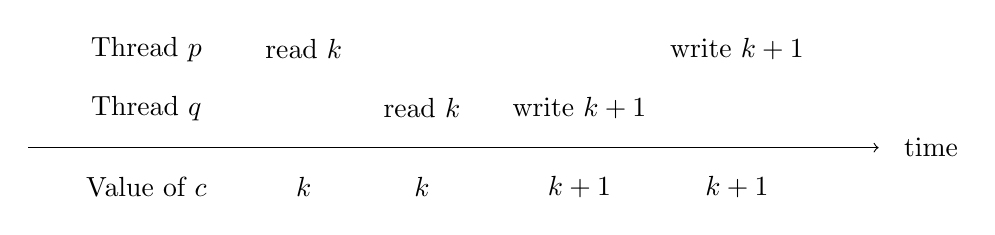
\begin{tikzpicture}
\node at (-1,0.75) {Thread $p$};
\node at (-1,0) {Thread $q$};
\node at (-1,-1){Value of $c$};

\node at (1,0.75) {read $k$};
\node at (1,-1) {$k$};

\node at (2.5,0.0) {read $k$};
\node at (2.5,-1) {$k$};

\node at (4.5,0) {write $k+1$};
\node at (4.5,-1) {$k+1$};

\node at (6.5,0.75) {write $k+1$};
\node at (6.5,-1) {$k+1$};

\draw[->] (-2.5, -0.5) -- (8.3, -0.5);

\node at (8.5, -0.5) [anchor=west]{time};
\end{tikzpicture}
\end{myimage}
\caption {Competition for access to a shared resource.}
\label{fig/competition}
\end{myfigure}
%
Assume the scenario described in figure~\ref {fig/competition}.
Thread $p$ reads the value of counter $c$, then gives control to $q$.
In its turn, $q$ reads the value of $c$, then writes the value $k+1$
to $c$.  The thread $p$ resumes control and writes the value $k+1$ to
$c$. The final value of $c$ is therefore $k+1$ instead of $k+2$.

This classic problem can be resolved by using locks that
prevent arbitrary interleaving of $p$ and $q$.

Locks are shared objects that can be held by at most a single thread
within a program at a time. A lock is created by the function
\pthreadcall[mutex]{create}.
%
\begin{codefile}{tmpmutex.mli}
  type t
\end{codefile}
%
\begin{listingcodefile}{tmpmutex.mli}
val $\libvalue{Mutex}{create}$ : unit -> t
\end{listingcodefile}
%
This operation a constructs a new lock, initially not held by any thread.
To acquire an existing lock, it is necessary to call the function
\pthreadcall[mutex]{lock} with the lock as argument. If the lock is
held by another thread, the caller is frozen until the lock is released.
A lock must be released explicitly by the thread that holds it, by
calling \pthreadcall[mutex]{unlock}.
%
\begin{listingcodefile}{tmpmutex.mli}
val $\libvalue{Mutex}{lock}$ : t -> unit
val $\libvalue{Mutex}{unlock}$ : t -> unit
\end{listingcodefile}
%
The \ml+lock+ call behaves like \ml+Thread.join+ with respect to
signals: if the thread receives a signal while executing \ml+lock+,
the signal will be noted ({\ie} the {\ocaml} runtime will be notified
that the signal has arrived), but the thread will continue to wait so
that \ml+lock+ effectively returns only when the lock has been
acquired, and never raises the \ml+EINTR+ exception.  The real
treatment of the signal by {\ocaml} will happen only upon the return
from \ml+lock+.

We can also try to acquire a lock without blocking by calling
\pthreadcall[mutex]{trylock}
%
\begin{listingcodefile}{tmpmutex.mli}
val $\libvalue{Mutex}{try\_lock}$ : t -> bool
\end{listingcodefile}
%
This function returns \ml+true+ if the lock has been acquired and
\ml+false+ otherwise.  In the latter case, execution is not suspended
since the lock is not acquired. The thread can therefore do something
else and eventually return and try its luck later.

\begin{example}

Incrementing a global counter used by several threads poses a
synchronization problem: the instants between reading the value of the
counter and writing the incremented value are in a critical region,
{\ie} two threads cannot be in this region at the same time. The
synchronization can easily be managed with a lock.
%
\begin{listingcodefile}{cthread.ml}
type counter = { lock : Mutex.t; mutable counter : int }
let newcounter() = { lock = Mutex.create(); counter = 0 }
let addtocounter c k = 
  Mutex.lock c.lock; 
  c.counter <- c.counter + k; 
  Mutex.unlock c.lock;;
\end{listingcodefile}
%
The sole read operation on the counter poses no problem. It can be
performed in parallel with a modification of the counter: the result
will simply be the value of the counter just before or just after the
modification, both results being consistent.
\end{example}

A common pattern is to hold a lock temporarily during a function call.
It is of course necessary to make sure to release the lock at the end
of the call, whether the call succeeded or failed. We can abstract
this behavior in a library function:
\begin{codefile}{misc.mli}
val run_with_lock : Mutex.t -> ('a -> 'b) -> 'a -> 'b
\end{codefile}
\begin{listingcodefile}{misc.ml}
let run_with_lock l f x = 
  Mutex.lock l; try_finalize f x Mutex.unlock l
\end{listingcodefile}
In the preceding example, we could also have written:
\begin{codefile}{cthread.ml}
open Misc;;
\end{codefile}
\begin{listingcodefile}{cthread.ml}
let addtocounter c =
  Misc.run_with_lock c.lock (fun k -> c.counter <- c.counter + k)
\end{listingcodefile}

\begin{example}
An alternative to the model of the server with threads is to start a
number of threads in advance which handle requests in parallel.
%
\begin{codefile}{farm.mli}
open Unix
\end{codefile}
%
\begin{listingcodefile}{farm.mli}
val tcp_farm_server : 
  int -> (file_descr -> file_descr * sockaddr -> 'a) -> sockaddr -> unit
\end{listingcodefile}
%
The \ml+tcp_farm_server+ function behaves like \ml+tcp_server+ but
takes an additional argument which is the number of threads to start,
each of which will become a server at the same address. The advantage
of a pool of threads is to reduce the time to handle each connection
by eliminating the cost of creating a thread for it, since they are
created once and for all.
%
\begin{codefile}{farm.ml}
open Sys;;
open Unix;;
\end{codefile}
%
\begin{listingcodefile}{farm.ml}
let tcp_farm_server n treat_connection addr = 
  let server_sock = Misc.install_tcp_server_socket addr in 
  let mutex = Mutex.create() in
  let rec serve () =
    let client = 
      Misc.run_with_lock mutex 
        (Misc.restart_on_EINTR accept) server_sock in
    treat_connection server_sock client;
    serve () in
  for i = 1 to n-1 do ignore (Thread.create serve ()) done;
  serve ();;
\end{listingcodefile}
The only precaution to take is to ensure mutual exclusion around the
\ml+accept+ so that only one of the threads accepts a connection at a
time. The idea is that the \ml+treat_connection+ function performs a
sequential treatment, but it is not a requirement~---~we can
effectively combine a pool of threads with the creation of new
threads, which can be dynamically adjusted depending on the load.
\end{example}

Acquisition of a lock is an inexpensive operation when it succeeds
without blocking. It is generally implemented with a single
\quotes{test-and-set} instruction provided by all modern processors
(plus other small costs that are involved, such as updating caches).
However, when the lock is not available, the process must be suspended
and rescheduled later, which involves a significant additional cost.
We must therefore incur this penalty only for a real suspension of a
process in order to give control to another, and not for its potential
suspension during the acquisition of a lock.  Consequently, we will
almost always want to release a lock as soon as possible and take it
back later if necessary, rather than simply holding onto the lock.
Avoiding these two operations would have the effect of enlarging the
critical region and therefore the frequency with which another thread
finds itself effectively in competition for the lock and in need of
suspension.

Locks reduce interleaving.  In return, they increase the risk of
deadlock.  For example, there is a deadlock if a thread $p$ waits for
a lock $v$ held by a thread $q$ which itself waits for a lock $u$ held
by $p$.  (In the worst case, a thread waits for a lock that it holds
itself.)  Concurrent programming is difficult, and guarding against
deadlock is not always easy.  A simple way of avoiding this situation
that is often possible consists of defining a hierarchy among the
locks and ensuring that the order in which the locks are acquired
dynamically respects the hierarchy: a thread never acquires a lock
unless that lock is dominated by all the other locks that the thread
already holds.

\section{Complete example: {\http} relay}
\label{ex/th-relais}

We will modify the {\http} relay developed in the preceding chapter
so that it services requests using threads.

Intuitively, it suffices to replace the \ml+establish_server+ function
that creates a process clone with a function that creates a
thread.  We must however take certain precautions.  The challenge
with threads is that they share the entire memory space.  We must
therefore ensure that the threads are not \quotes{stepping on each
other's toes} with one undoing what was just done by another.
That typically happens when two threads modify the same mutable
structure in parallel.

In the case of the {\http} server, there are several changes to make.
Let us start by resolving problems with access to resources.  The
\ml+proxy_service+ function, described in section~\ref{page/get_url},
handles the treatment of connections.  Via the intermediary functions
\ml+parse_host+, \ml+parse_url+ and \ml+parse_request+, it calls the
\ml+regexp_match+ function which uses the \ml+Str+ library.  However,
this library is not re-entrant (the result of the last search is
stored in a global variable). This example shows that we must beware
of calls to innocent-looking functions that hide potential collisions.
In this case we will not rewrite the \ml+Str+ library but simply
sequentialize its use.  It suffices to protect calls to this library
with locks (and there is really no other choice). We must still take
the precaution of releasing the lock when returning from the function
abnormally due to an exception.

To modify the existing code as little as possible, we can just rename
the definition of \ml+regexp_match+ in the \ml+Url+ module as
\ml+unsafe_regexp_match+ and then define \ml+regexp_match+ as a
protected version of \ml+unsafe_regexp_match+.
%
\begin{codefile}{thurl.ed}
f th/url.ml
r url.ml
/^let regexp_match/s/regexp_match/unsafe_regexp_match/
/^let/-1a
open Misc;;
\end{codefile}
%
\begin{listingcodefile}{thurl.ed}
let strlock = Mutex.create();;
let regexp_match r string =
  Misc.run_with_lock strlock (unsafe_regexp_match r) string;;
\end{listingcodefile}

The change is rather minimal.  It should be noted that the
\ml+regexp_match+ function includes both the expression matching and
the extraction of the matched groups.  It would definitely have been
incorrect to protect the \ml+Str.string_match+ and
\ml+Str.matched_group+ functions individually.

Another solution would be to rewrite the analysis functions without using
the \ml+Str+ library.  But there is no reason for such a choice, since
synchronizing the library primitives is easy to do and does not turn
out to be a source of inefficiency.  Obviously, a better solution
would be for the \ml+Str+ library to be re-entrant in the first place.

The other functions that are called are already re-entrant, in particular
the \ml+Misc.retransmit+ function that allocates different buffers for
each call.

However, there are still some precautions to take regarding error
handling.  The handling of a connection by a thread must be robust, as
explained above. In particular, in case of error, the other threads
must not be affected. In other words, the thread must terminate
\quotes{normally}, properly closing the connection in question and
going back to accepting other pending connections.  We must first of
all replace the call to \ml+exit+ in \ml+handle_error+ because it is
essential not to kill the whole process.  A call to \ml+Thread.exit+
would not be correct either, because thread termination does not close
its (shared) descriptors, the way the system does for process
termination.  An error in the handling of a connection would leave the
connection open.  The solution consists of raising an \ml+Exit+
exception that allows the finalization code to do what is required.
We must now protect \ml+treat_connection+ by catching all errors, in
particular \ml+Exit+ but also \ml+EPIPE+, which can be raised if the
client closes the connection prematurely.  We will take care of this
by using a protected function.
%
\begin{codefile}{thurl.ed}
.
1;#
/handle_error/;#
-1a
exception Exit;;
.
.,++s/exit 2/raise Exit/
wq
\end{codefile}
%
\begin{codefile}{thproxy.ed}
f th/proxy.ml
r proxy.ml
/let proxy/-1a
\end{codefile}
\begin{listingcodefile}{thproxy.ed}
let allow_connection_errors f s = 
  try f s with Exit | Unix_error(EPIPE,_,_) -> ()
\end{listingcodefile}
%
\begin{codefile}{thproxy.ed}
.
/let treat_connection/c
\end{codefile}
%
\begin{listingcodefile}{thproxy.ed}
let treat_connection s = 
  Misc.co_treatment s (allow_connection_errors proxy_service) in
\end{listingcodefile}
%
\begin{codefile}{thproxy.ed}
.
wq
\end{codefile}

\begin{exercise}[noanswer]
Rewrite the proxy for the {\http}/1.1 protocol using threads.
\end{exercise}

\begin{exercise}[noanswer]
Coroutines can be seen as a very particular kind of threads where each
process must surrender control explicitly before another can execute.
Give an implementation of coroutines using threads.
\end{exercise}

\section{Conditions}

The functions described in this section are defined in the
\libmodule{Condition} module.

Synchronization with locks is very simple, but it is not sufficient:
locks allow waiting for shared data to be free, but do not allow
waiting for the data to have a particular state.  Let us replace the
example of a counter by a (first-in/first-out) queue shared among
several threads.  Adding a value to the queue can be synchronized by
using a lock as above, since no matter what the state of the queue,
we can always add an element.  But what about removing an element
from the queue?  What should be done when the queue is empty?  We
cannot hold the lock while waiting for the queue to be filled, because
that would completely prevent another thread from filling the queue.
So it must be released.  But how can we know when the queue is no
longer empty, except by testing it periodically?  This solution,
called \quotes{busy-waiting}, is definitely not satisfactory.  Either
it consumes computing cycles unnecessarily (period too short) or else
it it is not reactive enough (period too long).

\emph{Conditions} provide a solution to this problem.  A thread that
holds a lock can wait for a condition object until another thread
sends a signal on that condition.  As with locks, conditions are
passive structures that can be manipulated by synchronization
functions.  They can be created by the \pthreadcall[cond]{create}
function.
%
\begin{codefile}{tmpcondition.mli}
type t
\end{codefile}
%
\begin{listingcodefile}{tmpcondition.mli}
val $\libvalue{Condition}{create}$ : unit -> t
\end{listingcodefile}
%
A process $p$ that \emph{already holds} a lock \ml+v+ can wait on a
condition \ml+c+ and the \ml+v+ by calling \pthreadcall[cond]{wait}.
The process $p$ informs the system that it is waiting on the condition
\ml+c+ and the lock \ml+v+, then releases the lock \ml+v+ and goes to
sleep.  It will not be woken up by the system until another thread $q$
signals a change on the condition \ml+c+ and the lock \ml+v+ is
available; the process $p$ will then hold the lock \ml+v+ again.
%
\begin{listingcodefile}{tmpcondition.mli}
val $\libvalue{Condition}{wait}$ : t -> Mutex.t -> unit
\end{listingcodefile}
%
Note: it is an error to call \ml+wait c v+ without holding the lock
\ml+v+.  The behavior of \ml+wait c v+ with respect to signals is the
same as for \ml+Mutex.lock+.

When a thread signals a change on a condition, it can either ask for
all threads waiting on that condition to be woken up
(\pthreadcall[cond]{broadcast}), or else for just one of them to be
woken up (\pthreadcall[cond]{signal}).
%
\begin{listingcodefile}{tmpcondition.mli}
val $\libvalue{Condition}{signal}$ : t -> unit
val $\libvalue{Condition}{broadcast}$ : t -> unit
\end{listingcodefile}
%
Sending a signal or a broadcast on a condition does not require
holding a lock (unlike waiting), in the sense that it will not trigger
a \quotes{system} error.
%%
%% Est-ce vrai? c'est � celui qui se met en attente � avoir pris le verrou
%% avant de tester, puis fait wait. Il est donc s�r que la condition n'est
%% pas vrai � ce moment l�. 
%% 
However, it can sometimes be a programming error.
%% En effet, �mettre un signal sans poss�der le verrou sur
%% lequel les r�cepteurs de ce signal sont en attente signifie que
%% l'�mission du signal n'est pas synchronis�e avec la mise en attente et
%% peut donc se produire avant la mise en attente qu'il est suppos�
%% interrompre: le signal sera alors ignor� et l'attente jamais
%% interrompue (voir l'exemple des queues ci-dessous).  

The choice between waking up one thread or all the threads depends on
the problem.  To consider the example of the queue again, if a thread
adds an element to an empty queue, there is no need to wake up all the
others, since only one will effectively be able to remove that
element.  On the other hand, if it adds a number of elements that is
either not statically known or very large, it must wake up all the
threads.  Note that if adding an element to a non-empty queue does not
send a signal, then adding an element to an empty queue must send a
broadcast, since it could be followed immediately by another addition
(without a signal) and therefore behave like a multiple addition.
In summary, either send a signal on every addition, or send a
broadcast only when adding to an empty queue.
The choice between these two strategies is a bet on whether the queue
is usually empty (first solution) or usually non-empty (second
solution).

Often, one thread knows only an approximation of the reason why
another thread is waiting on a condition.  It will therefore signal
the condition whenever the situation \emph{might} be what the other
thread is waiting for.  An awakened thread, therefore, cannot assume
that the condition it was waiting is now satisfied.  It must, in
general, re-test the state of its shared data, and if necessary wait
on the condition again.  This does not constitute busy-waiting, because
it only happens when another thread signals the condition.

Here is another justification for this approach: when a thread has
just produced a lot of some resource and wakes all the others using a
\ml+broadcast+, nothing prevents the first one that wakes up from
being greedy and exhausting the entire resource.  The second one to
wake up must go back to sleep, hoping to be luckier next time.

We can now give a concrete solution for shared queues.  The \ml+queue+
structure defined in the \ml+Queue+ module is extended with a lock and
a \ml+non_empty+ condition.
%
\begin{listingcodefile}[style=numbers]{thcheck.ml}
type 'a t = 
  { queue : 'a Queue.t; lock : Mutex.t; non_empty : Condition.t }
let create () = 
  { queue = Queue.create(); 
    lock = Mutex.create(); non_empty = Condition.create() }

let add e q = 
  Mutex.lock q.lock; 
  if Queue.length q.queue = 0 then Condition.broadcast q.non_empty;$\label{prog:broadcast}$
  Queue.add e q.queue; 
  Mutex.unlock q.lock;;

let take q = 
  Mutex.lock q.lock; 
  while Queue.length q.queue = 0 $\label{prog:lock}$
  do Condition.wait q.non_empty q.lock done;  $\label{prog:slock}$
  let x = Queue.take q.queue in
  Mutex.unlock q.lock; x;;
\end{listingcodefile}
%
Addition never blocks, but we must not forget to signal
the \ml+non_empty+ condition when the list is empty beforehand,
because it is possible that someone is waiting on the condition.

Removal is a little more complicated: after acquiring the lock, we
must try to remove an element from the queue. If the queue is empty,
we must wait on the \ml+non_empty+ condition.  When awakened, we try
again, knowing that we already have the lock.

As explained above, the \ml+broadcast q.non_empty+ signal
(line~\ref{prog:broadcast}) is executed by a thread $p$ already in
possession of the lock \ml+q.lock+.
This implies that a reader thread $q$ executing the \ml+take+ function
cannot be between line~\ref{prog:lock} and~\ref{prog:slock}
where it would have verified that the queue is empty but not yet have
gone to sleep.  In this case, the signal sent by $p$ would be
ineffective and ignored, since $q$ has not gone to sleep yet; but $q$
would then go to sleep and not be woken up, because $p$ has already
sent its signal.
The lock therefore guarantees that either $q$ is already asleep or
else has not yet tested the state of the queue.

\begin{exercise}
Implement a variant in which the queue is bounded: addition to the
queue becomes blocking when the size of the queue reaches a fixed
value. (In a concurrent world, we might need this scheme to avoid
having a producer that produces endlessly while the consumer is
blocked.)
\end{exercise}
\begin{answer}
We must introduce an additional \ml+non_full+ condition.
We also add a \ml+size+ field to allow queues of different sizes.
%
\begin{listingcodefile}{thtqueue.ml}
type 'a t = 
    { queue : 'a Queue.t; size : int; lock : Mutex.t;
      non_empty : Condition.t; non_full : Condition.t; }
      
let create k = 
  if  k > 0 then
    { queue = Queue. create(); size = k; lock = Mutex. create(); 
      non_empty = Condition. create(); non_full = Condition.create() }
  else failwith "Tqueue.create: empty size";;
\end{listingcodefile}
%
Addition is a combination of the preceding versions of the
\ml+add+ and \ml+take+ functions above.
%
\begin{listingcodefile}{thtqueue.ml}
let add x q = 
  Mutex.lock q.lock;
  while Queue.length q.queue = q.size 
  do Condition.wait q.non_full q.lock done;
  if Queue.is_empty q.queue then Condition.broadcast q.non_empty;
  Queue.add q x;
  Mutex.unlock q.lock;;
\end{listingcodefile}
%
Removal is symmetric to addition (and must now signal \ml+non_full+
when the queue is full beforehand), and is left to the reader.
%
\begin{codefile}{thtqueue.ml}
let take q = 
  Mutex.lock q.lock;
  while Queue.length q.queue = 0 
  do Condition.wait q.non_empty q.lock done;
  if Queue.length q.queue = q.size then Condition.broadcast q.non_full;
  let x = Queue.take q.queue in
  Mutex.unlock q.lock; x;;
\end{codefile}
%
We get the behavior of unbounded queues by choosing \ml+max_int+ for
\ml+size+.
\end{answer}



\section{Event-based synchronous communication}

The functions described in this section are defined in the
\libmodule{Event} module.

Locks and conditions together allow all forms of synchronization to be
expressed.  However, their implementation is not always easy, as shown
by the example of the initially simple queue whose synchronization
code subsequently turned out to be subtle.

Event-based synchronous communication is a collection of higher-level
communication primitives that tend to facilitate concurrent
programming.  The primitives in the \ml+Event+ module were initially
developed by John Reppy as an extension of the \emph{Standard ML}
language called \emph{Concurrent ML}~\cite{CML}.  In {\ocaml}, these
primitives are located above the more elementary synchronization of
locks and conditions.

Communication occurs by sending \emph{events} along \emph{channels}.
Channels are like \quotes{lightweight pipes}: they allow communication
among threads in the same program and take care of synchronization
between producers and consumers.  A channel carrying values of type
\ml+'a+ has the type \ml+'a Event.channel+.  Channels are homogeneous
and therefore always carry values of the same type.  A channel is
created with the \ml+new_channel+ primitive.
%
\begin{codefile}{tmpevent.mli}
type 'a channel
type +'a event
\end{codefile}
%
\begin{listingcodefile}{tmpevent.mli}
val $\indexlibvalue{Event}{new\_channel}$ : unit -> 'a channel
\end{listingcodefile}
%
Sending or receiving a message is not done directly, but through the
intermediary of an event.  An elementary event is \quotes{sending a
message} or \quotes{receiving a message}.  They are constructed by
means of the following primitives:
%
\begin{listingcodefile}{tmpevent.mli}
val $\indexlibvalue{Event}{send}$ : 'a channel -> 'a -> unit event
val $\indexlibvalue{Event}{receive}$ : 'a channel -> 'a event
\end{listingcodefile}
%
Construction of a message does not have an immediate effect: it just
creates a data structure describing the action to be done.  To make an
event happen, the thread must synchronize with another thread wishing
to make the complementary event happen.  The \ml+sync+ primitive
allows a thread to wait for the occurrence of the event passed
as argument.
%
\begin{listingcodefile}{tmpevent.mli}
val $\indexlibvalue{Event}{sync}$ : 'a event -> 'a
\end{listingcodefile}
%
Thus, to send a value \ml+v+ on the channel \ml+c+, one can execute
\ml+sync (send c v)+.  The thread is suspended until the event occurs,
that is to say until another thread is ready to receive a value on the
channel \ml+c+.  In a symmetric fashion, a thread can wait for a
message on channel \ml+c+ by performing \ml+sync (receive c)+.

There is a competition among all the producers on one hand and all the
consumers on the other.  For example, if several threads try to send a
message on a channel but only one is ready to read it, it is clear
that only one producer will make the event occur.  The others will
remain suspended, without even noticing that another was
\quotes{served} ahead of them.

The competition can also occur within the same thread.
Multiple events can be combined by the \ml+choose+ primitive.
%
\begin{listingcodefile}{tmpevent.mli}
val $\indexlibvalue{Event}{choose}$ : 'a event list -> 'a event
\end{listingcodefile}
%
The resulting event is an offer, in parallel, of the events passed as
arguments, and occurs when exactly one of them occurs.  We distinguish
between the offer of an event and its occurrence.  The call
\ml+sync (choose [e1; e2])+ synchronizes by offering a choice of two events
\ml+e1+ and \ml+e2+, but only one of the two events will effectively
occur (the offer of the other event will be simultaneously canceled).
The \ml+wrap_abort+ primitive allows an event to handle being
canceled.
%
\begin{listingcodefile}{tmpevent.mli}
val $\indexlibvalue{Event}{wrap\_abort}$ : 'a event -> (unit -> unit) -> 'a event
\end{listingcodefile}
%
The call \ml+wrap_abort e f+ creates an event that is equivalent to
\ml+e+, but if it is not chosen during synchronization, then the
function \ml+f+ is executed.  (This is only interesting when it is
part of a complex event.)

A thread can try to synchronize on an event without blocking (somewhat
like \ml+Mutex.try_lock+) with \ml+poll+.
%
\begin{listingcodefile}{tmpevent.mli}
val $\indexlibvalue{Event}{poll}$ : 'a event -> 'a option
\end{listingcodefile}
%
The call \ml+poll e+ offers the event \ml+e+ but if it cannot occur
immediately, it cancels the offer rather than blocking and has no
effect (or more exactly, behaves as if the expression \ml+poll e+ had
been replaced by the value \ml+None+).  By contrast, if the event can
happen immediately, then it behaves as if the thread had done
\ml+sync e+, except that the value \ml+Some v+ is returned
rather than \ml+v+.

\begin{example}
In example~\ref {ex/crible-copro} of the Sieve of Eratosthenes,
the communication between different threads is done with pipes as in
the original program, using system memory (the pipe) as intermediary.
One might think that it would be more efficient to communicate
directly by using the memory of the process.  A simple solution
consists of replacing the pipe by a channel on which integers are sent.

Sending integers on the channel is not sufficient, because we must
also be able to detect the end of the stream.  The simplest is
therefore to pass elements of the form \ml+Some n+ and to terminate by
sending the value \ml+None+.  To minimize the changes, we will go back
to the code in example~\ref{ex/crible}.  We simulate pipes and the
functions for reading and writing pipes by channels and functions for
reading and writing channels.

It is sufficient to take the previous version of the program and
change the input/output functions to ones that read and write a channel,
rather than an input/output buffer from the \ml+Pervasives+ library.
For example, we can insert the following code at line~2:
%
\begin{codefile}{theventcrible.ed}
f th/eventcrible.ml
r th/crible.ml
/let input_int/d
/let output_int/d
/generate/-1a
\end{codefile}
%
\begin{listingcodefile}{theventcrible.ed}
let pipe () = let c = Event.new_channel() in c, c
let out_channel_of_descr x = x
let in_channel_of_descr x = x

let input_int chan = 
  match Event.sync (Event.receive chan) with
  | Some v -> v 
  | None -> raise End_of_file
let output_int chan x = Event.sync (Event.send chan (Some x))
let close_out chan = Event.sync (Event.send chan None);;
\end{listingcodefile}
%
\begin{codefile}{theventcrible.ed}
.
wq
\end{codefile}

However, if we compare the efficiency of this version with the
previous one, we find that it is twice as slow.  Communication of each
integer requires a synchronization between two threads and therefore
several system calls for acquiring and releasing locks.  On the other
hand, communication via pipes uses buffered \io{} that allows several
thousand integers to be exchanged with each system call.

To be fair, one should also provide buffered communication on
channels, using the channel only to exchange a packet of integers.
The child can accumulate the results in a private queue, to which it
can therefore write without synchronization.  When the queue is full,
or upon an explicit request, it is emptied by synchronizing on the
channel.  The parent has its own queue that it receives by
synchronizing and empties gradually.

Here is a solution:
%
\begin{codefile}{thbuffercrible.ed}
f th/buffercrible.ml
r th/crible.ml
/generate/-1a
\end{codefile}
%
\begin{listingcodefile}{thbuffercrible.ed}
type 'a buffered = 
    { c : 'a Queue.t Event.channel; 
      mutable q : 'a Queue.t; 
      size : int }

let pipe () = let c = Event.new_channel() in c, c;;

let size = 1024;;
let out_channel_of_descr chan = 
  { c = chan; q = Queue.create(); size = size };;
let in_channel_of_descr = out_channel_of_descr;;

let input_int chan = 
  if Queue.length chan.q = 0 then begin
    let q = Event.sync (Event.receive chan.c) in
    if Queue.length q > 0 then chan.q <- q
    else raise End_of_file
  end;
  Queue.take chan.q;;

let flush_out chan = 
  if Queue.length chan.q > 0 then Event.sync (Event.send chan.c chan.q);
  chan.q <- Queue.create();;

let output_int chan x = 
  if Queue.length chan.q = size then flush_out chan;
  Queue.add x chan.q

let close_out chan = 
  flush_out chan;
  Event.sync (Event.send chan.c chan.q);;
\end{listingcodefile}
%
\begin{codefile}{thbuffercrible.ed}
.
wq
\end{codefile}
%
This version allows us to regain efficiency comparable to (but not
better than) the version with pipes.

Compared to the original version with processes and pipes, there are
two potential advantages. First, threads are more lightweight and less
costly to launch.  Second, communication on a channel merely passes a
pointer, without copying.  But these advantages are not noticeable
here, because the number of threads created and the data exchanged are
not big enough compared to the cost of system calls and compute time.

In conclusion, we can say that communication between threads has a
cost of up to one system call (if the process must be suspended) and
the cost can be significantly reduced by buffering communication and
sending larger structures less often.
\end{example}

\begin{exercise}[noanswer]
An {\http} server can be subjected to a high, bursty load.  To improve
response time, we can refine the architecture of an {\http} server by
always keeping a dozen threads ready to handle new requests. This means
that a thread does not handle only a single request, but a potentially
infinite series of requests that it reads from a queue.

To avoid overloading the machine, we can limit the number of threads
to a reasonable value beyond which the overhead of managing tasks
exceeds the latency for servicing requests (time spent waiting for
data on disk, \etc).  After that, we can keep some connections waiting
to be handled, and then finally we can refuse connections.  When the
load diminishes and the number of threads is above the \quotes{ideal}
value, some of them are allowed to die and the others remain ready for
the next requests.

Transform example~\ref{ex/th-relais} into this architecture.
\end{exercise}


\section{Implementation details}

\paragraph {Implementation of threads in Unix}

The Unix system was not originally designed to provide support for
threads.  However, most modern Unix implementations now offer such
support.  Nevertheless, threads remain an add-on that is sometimes
apparent.  For example, when using threads it is strongly discouraged
to use \ml+fork+ except when doing \ml+exec+ immediately afterward.
In effect, \ml+fork+ copies the current thread, which becomes a
crippled process that runs believing it has threads when in fact they
do not exist.  The parent continues to run normally as before.
The special case of a call to \ml+fork+ where the child immediately
launches another program does not cause the parent any problem.
Luckily, since that is the only way to start other programs!

Inversely, one can do \ml+fork+ (not followed by \ml+exec+), and then launch
several threads in the child and the parent, without any problem.

\paragraph {Native and simulated implementation in {\ocaml}}
\label{sec/thread-implementation}

When the underlying operating system has threads, {\ocaml} can provide
a native implementation of threads, leaving their management to the
operating system as much as possible.  Each thread then lives in a
different Unix process but shares the same address space.

When the system does not provide support for threads, {\ocaml} can
emulate them.  All the threads then execute in the same Unix process,
and their management, including their scheduling, is handled by the
{\ocaml} runtime system.  However, this implementation is only
available when compiling to bytecode.

The {\ocaml} system provides the same programming interface for the
native and simulated versions of threads. The implementation of
threads is therefore split: one implementation for the emulated
version that includes its own task controller, and another
implementation that is based on \textsc{posix}~(1003.1c) threads and
lifts the corresponding library functions to the level of the {\ocaml}
language.  In the process, the {\ocaml} language handles certain
simple administrative tasks and ensures an interface identical to the
emulated version.  This guarantees that a program compilable on one
Unix architecture remains compilable on another Unix architecture.
However, whether threads are emulated or native can change the
synchronization of calls to the C library, and therefore change,
despite everything, the semantics of the program.  It is therefore
necessary to take certain precautions before believing that a program
will behave the same way in these two versions.  In this chapter, the
discussion will mainly concern these two implementations, but recall
that by default, we have taken the viewpoint of a native
implementation.

To use emulated threads, one must pass the \ml+-vmthreads+ option
instead of \ml+-threads+ to the \ml+ocamlc+ compiler. This option is
not accepted by the \ml+ocamlopt+ compiler.

\paragraph{Sequentialization of {\ocaml} code}

The implementation of threads in {\ocaml} must face one of the
peculiarities of the {\ocaml} language: the automatic management of
memory and its high consumption of allocated data.  The solution
adopted, which is the simplest and also generally the most efficient,
is to sequentialize the execution of {\ocaml} code in all threads: a
lock in the runtime system prevents two threads from executing
{\ocaml} code simultaneously.  This seems contrary to the whole idea
of threads, but it is not, since the lock is released before blocking
system calls and reacquired upon return.  Other threads can therefore
take control at that moment.  A special case of such a system call is
the call to \ml+sched_yield+, performed at regular intervals to
suspend the running thread and give control to another.

On a multiprocessor machine, the only source of true parallelism comes
from the execution of C code and system calls.  On a uniprocessor
machine, the fact that the {\ocaml} code is sequentialized is not
really noticeable.

The programmer cannot rely on this sequentialization, because one
thread can give control to another at almost any moment.  With one
exception, the sequentialization guarantees memory coherence: two
threads always have the same view of memory, except perhaps when they
execute C code.  In effect, the passing of the lock implies a
synchronization of the memory: a read operation by one thread
occurring after a write operation to the same address by another
thread will always return the freshly-written value, with no need for
additional synchronization.

\paragraph {Threads and signals}

Generally speaking, using signals is already delicate with a single
thread due to their asynchronous character.  It is even more so in the
presence of multiple threads because of the addition of new
difficulties: which thread should a signal be sent to?  To all, to the
primary one, or to the one currently running?  What happens if one
thread sends a signal to another?  In fact, threads were implemented
before answering these questions, and different implementations can
behave differently with respect to signals.

The \ml+Thread.join+, \ml+Mutex.lock+, and \ml+Condition.wait+,
despite being long system calls, are not interruptible by a signal.
(They cannot therefore fail with the \ml+EINTR+ error.)  If a signal
is sent while waiting, it will be received and handled when the call
returns.

The \textsc{posix} standard specifies that the signal handler is
shared among all the threads and in contrast the signal mask is
private to each thread and inherited upon creation of a thread.  But
the behavior of threads with respect to signals remains largely
underspecified and therefore non-portable.

It is therefore preferable to avoid as much as possible the use of
asynchronous signals (such as \ml+sigalrm+, \ml+sigvtalrm+,
\ml+sigchld+, \etc) with threads. These can be blocked and examined
with \ml+Thread.wait_signal+.  One can dedicate a thread to signal
handling and nothing else: it can wait for the reception of signals,
undertake the necessary actions, and update certain information
examined by other threads.

In addition, {\ocaml} threads (since version 3.08) use the
\ml+sigvtalarm+ signal internally to implement preemption of threads.
This signal is therefore reserved and must not be used by the program
itself, since there is a risk of interference.

\begin{codefile}{thmisc.ed}
f th/misc.mli
r misc.mli
$r th/misc.MLI
w
f th/misc.ml
1,$ d
r misc.ml
$r th/misc.ML
wq
\end{codefile}






